\documentclass[11pt,a4paper]{article}
\usepackage[utf8]{inputenc}
\usepackage[T1]{fontenc}
\usepackage[spanish]{babel}
\usepackage{lmodern}
\usepackage{geometry}
\usepackage{graphicx}
\usepackage{booktabs}
\usepackage{amsmath}
\usepackage{float}
\usepackage{xcolor}
\usepackage{hyperref}
\geometry{margin=2.4cm}
\hypersetup{colorlinks=true,linkcolor=blue,urlcolor=blue}
\newcommand{\codigo}[1]{\texttt{#1}}
\title{Laboratorio 09\\Bag of Words, similitud de coseno e índice invertido}
\author{Juan Marcos Guerrero Cueva\\Base de Datos II\\Prof. Heider Sánchez}
\date{16 de octubre de 2026}
\begin{document}
\maketitle
\begin{abstract}
Se implementaron y compararon cuatro rutas de recuperación textual sobre 1217
noticias reales. El informe presenta el preprocesamiento, la validación de resultados,
mediciones repetidas sobre seis tamaños de colección y un análisis sustentado por los CSV
entregados con el código.
\end{abstract}
\tableofcontents
\clearpage

\section{P1. Configuración y carga de datos}
Se utilizó PostgreSQL 18.6 en Windows-\allowbreak{}11-\allowbreak{}10.0.26200-\allowbreak{}SP0, Python 3.14.7, pandas
3.0.6, NLTK 3.10.3 y Matplotlib 3.11.2. La tabla
\codigo{noticias} tiene columnas \codigo{id}, \codigo{url}, \codigo{contenido},
\codigo{categoria} y \codigo{bag\_of\_words JSONB}; \codigo{stopwords} tiene
\codigo{id} y \codigo{word UNIQUE}. \codigo{crear\_bd.py} crea las tablas si no
existen y \codigo{carga.py} importa \codigo{news\_es.csv} y \codigo{stoplist.txt}
solo cuando las tablas están vacías. Se verificaron 1217 noticias y
608 stopwords. Los identificadores de noticias van de 1 a 1217. No se
duplicó la carga ya presente. La conexión se toma de \codigo{.env}, que Git ignora.

\section{P2. Preprocesamiento y Bag of Words}
\codigo{preprocess(text)} pasa a minúsculas, extrae secuencias de letras Unicode,
elimina las stopwords leídas de PostgreSQL y aplica \codigo{SnowballStemmer}
en español. Se conservan las tildes; signos y números se descartan. \codigo{NULL}
y texto vacío producen una lista vacía. \codigo{compute\_bow(text)} cuenta cada
término resultante. Por ejemplo, ``Banco, banco! 123'' produce
\codigo{\{'banc': 2\}}. La misma función normaliza documentos y consultas.
\codigo{update\_bow\_in\_db(dataframe)} guarda cada diccionario como JSONB
con parámetros SQL y una transacción. La función \codigo{fetch\_data\_bow()}
lee \codigo{noticias}; el comentario del enunciado sobre \codigo{noticias\_bow}
no corresponde a una tabla creada. Se verificó que los 1217 BoW son no nulos.
\begin{verbatim}
tokens = preprocess(text)
bow = dict(Counter(tokens))
UPDATE noticias SET bag_of_words = %s WHERE id = %s
\end{verbatim}
El script de ejecución muestra las primeras diez filas abreviadas. La validación
incluye el texto vacío, una frecuencia conocida y una consulta sin términos presentes.

\section{P3. Búsqueda booleana}
\codigo{boolean\_search\_linear} evalúa cada BoW. \codigo{InvertedIndex}
construye listas \codigo{(doc\_id, tf)} y resuelve \codigo{AND}, \codigo{OR}
y \codigo{AND\_NOT} mediante intersección, unión y diferencia de IDs. El analizador
acepta paréntesis y da prioridad a \codigo{AND} y \codigo{AND-NOT} sobre
\codigo{OR}. Ambos métodos devuelven IDs únicos ordenados de forma ascendente.
\begin{table}[H]\centering\small
\begin{tabular}{p{0.6cm}p{8.8cm}rr}\toprule
Nº & Consulta & Coincidencias & ¿Iguales?\\\midrule
1 & economía AND inflación & 244 & Sí \\
2 & banca OR finanzas & 547 & Sí \\
3 & tecnología AND-NOT inflación & 306 & Sí \\
4 & sostenibilidad AND ambiente AND renovables & 9 & Sí \\
5 & tecnología AND (banca OR finanzas) & 174 & Sí \\
6 & economía AND-NOT inflación & 358 & Sí \\
\bottomrule\end{tabular}
\caption{Seis pruebas booleanas sobre los 1217 documentos.}
\end{table}

\section{P4. Similitud de coseno}
Para un término $t$ en una colección de $N$ documentos se usó
$\mathrm{idf}(t)=\ln((N+1)/(\mathrm{df}(t)+1))+1$ y
$w_{t,d}=\mathrm{tf}(t,d)\,\mathrm{idf}(t)$.
El score es $\sum_t w_{t,q}w_{t,d}/(\lVert q\rVert_2\lVert d\rVert_2)$.
Las dos rutas comparten IDF y normas. La lineal examina todos los BoW; la del
índice acumula solamente documentos en las listas de términos de la consulta.
Se ordena por score descendente e ID ascendente. Si no hay coincidencias o la
norma es cero, se devuelve lista vacía. Un \codigo{top\_k} grande devuelve los
candidatos existentes.
\begin{table}[H]\centering\footnotesize
\begin{tabular}{p{4.5cm}p{4.2cm}p{5cm}}\toprule
Consulta & IDs top 5 & Scores top 5\\\midrule
innovaciones en banca digital y tecnología financiera & 390, 259, 220, 282, 394 & 0.4229, 0.4137, 0.3840, 0.3564, 0.3183 \\
inflación y crecimiento económico & 108, 510, 368, 803, 926 & 0.3483, 0.3407, 0.3337, 0.3336, 0.3311 \\
sostenibilidad y energías renovables & 523, 150, 677, 661, 1106 & 0.5052, 0.4968, 0.3036, 0.2831, 0.2543 \\
\bottomrule\end{tabular}
\caption{Resultados reales; ambas rutas dieron los mismos IDs y scores con tolerancia $10^{-12}$.}
\end{table}

\section{P5. Experimento y gráficos}
Se tomaron los primeros $N$ documentos por ID ascendente, con tamaños
122, 304, 487, 730, 974, 1217. Para cada tamaño se construyó un índice propio sobre exactamente el
mismo subconjunto usado por la ruta lineal. Se verificó la igualdad de resultados
antes de medir. Se hizo un calentamiento y luego 30 repeticiones de cada
una de las seis consultas booleanas y tres de coseno. Se midió con
\codigo{time.perf\_counter()}; el CSV crudo guarda una fila por ejecución.
Cada punto es el promedio de todas las consultas y repeticiones del tipo indicado.
El tiempo de construcción se informa aparte. El BoW, IDF y normas estaban
preparados antes de cronometrar consultas. El orden de ejecución fue fijo;
las variaciones del sistema pueden afectar los microtiempos.
\begin{table}[H]\centering\small
\begin{tabular}{rrrrr}\toprule
$N$ & Booleano lineal & Booleano índice & Coseno lineal & Coseno índice\\\midrule
122 & 0.000382 & 0.000051 & 0.000220 & 0.000085 \\
304 & 0.000671 & 0.000078 & 0.000490 & 0.000161 \\
487 & 0.000893 & 0.000095 & 0.000815 & 0.000251 \\
730 & 0.001219 & 0.000125 & 0.001186 & 0.000364 \\
974 & 0.001971 & 0.000190 & 0.001923 & 0.000585 \\
1217 & 0.004404 & 0.000441 & 0.004318 & 0.001308 \\
\bottomrule\end{tabular}
\caption{Tiempo promedio por consulta en segundos; fuente: \codigo{resultados/promedios.csv}.}
\end{table}
\begin{table}[H]\centering\small
\begin{tabular}{rrrr}\toprule
$N$ & Construcción (s) & Términos & Postings\\\midrule
122 & 0.01200 & 4449 & 17783 \\
304 & 0.05108 & 7096 & 45757 \\
487 & 0.03037 & 8938 & 72849 \\
730 & 0.04849 & 10660 & 108491 \\
974 & 0.09604 & 11990 & 143323 \\
1217 & 0.16528 & 13343 & 180216 \\
\bottomrule\end{tabular}
\caption{Costo y tamaño del índice en memoria; fuente: \codigo{resultados/construccion\_indice.csv}.}
\end{table}
\begin{figure}[H]\centering
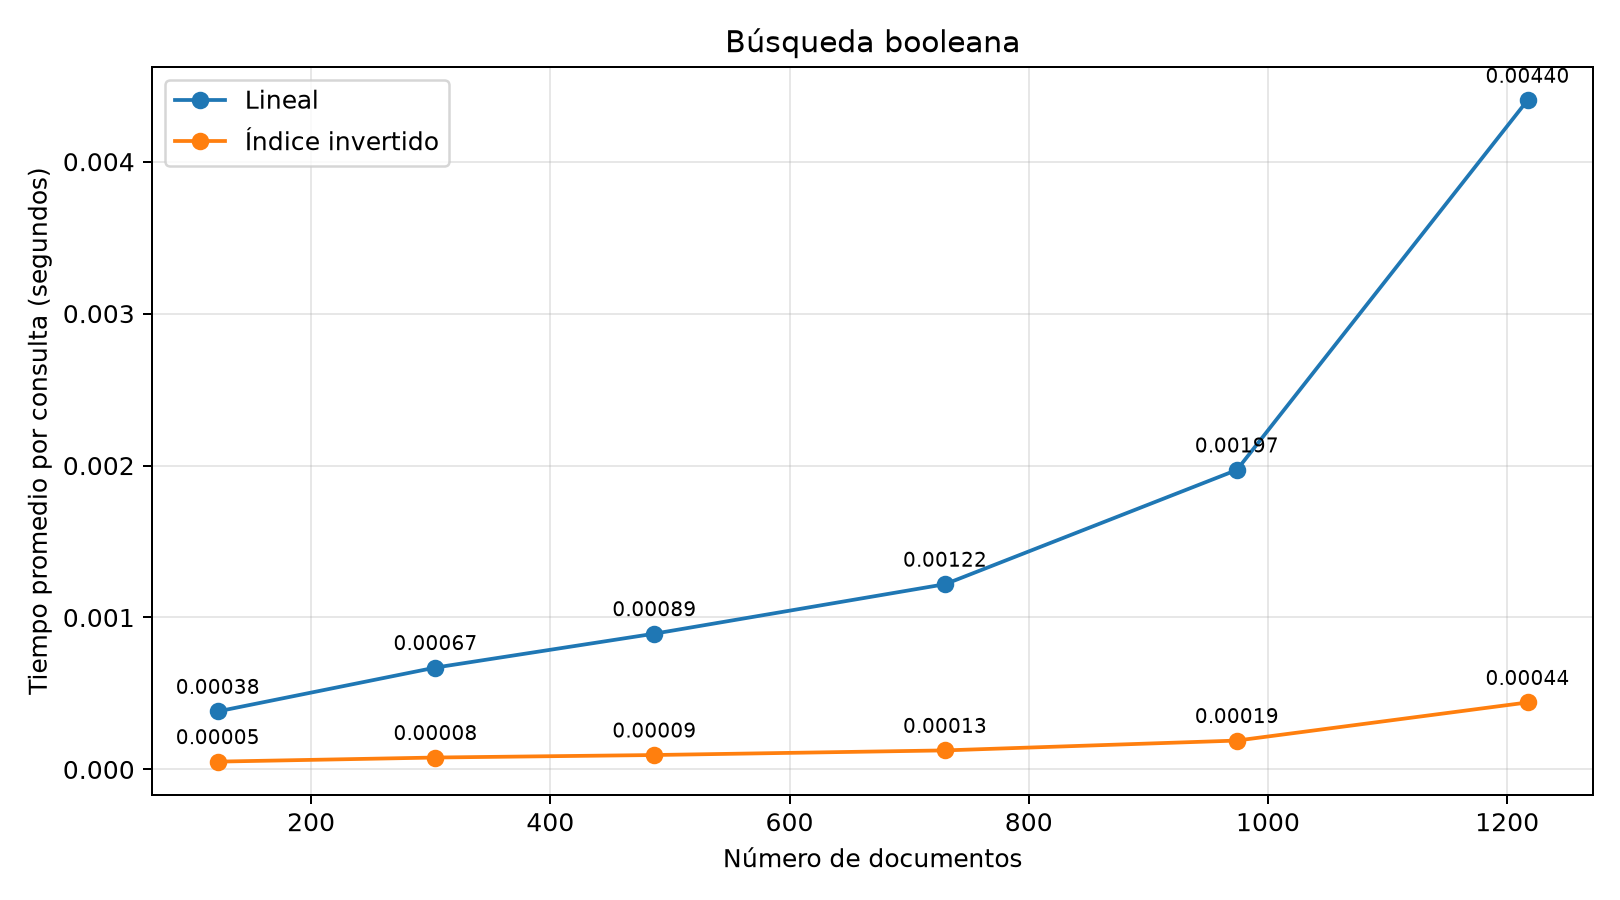
\includegraphics[width=0.95\linewidth]{resultados/booleana.png}
\caption{Tiempo promedio de la búsqueda booleana; construcción excluida.}
\end{figure}
\begin{figure}[H]\centering
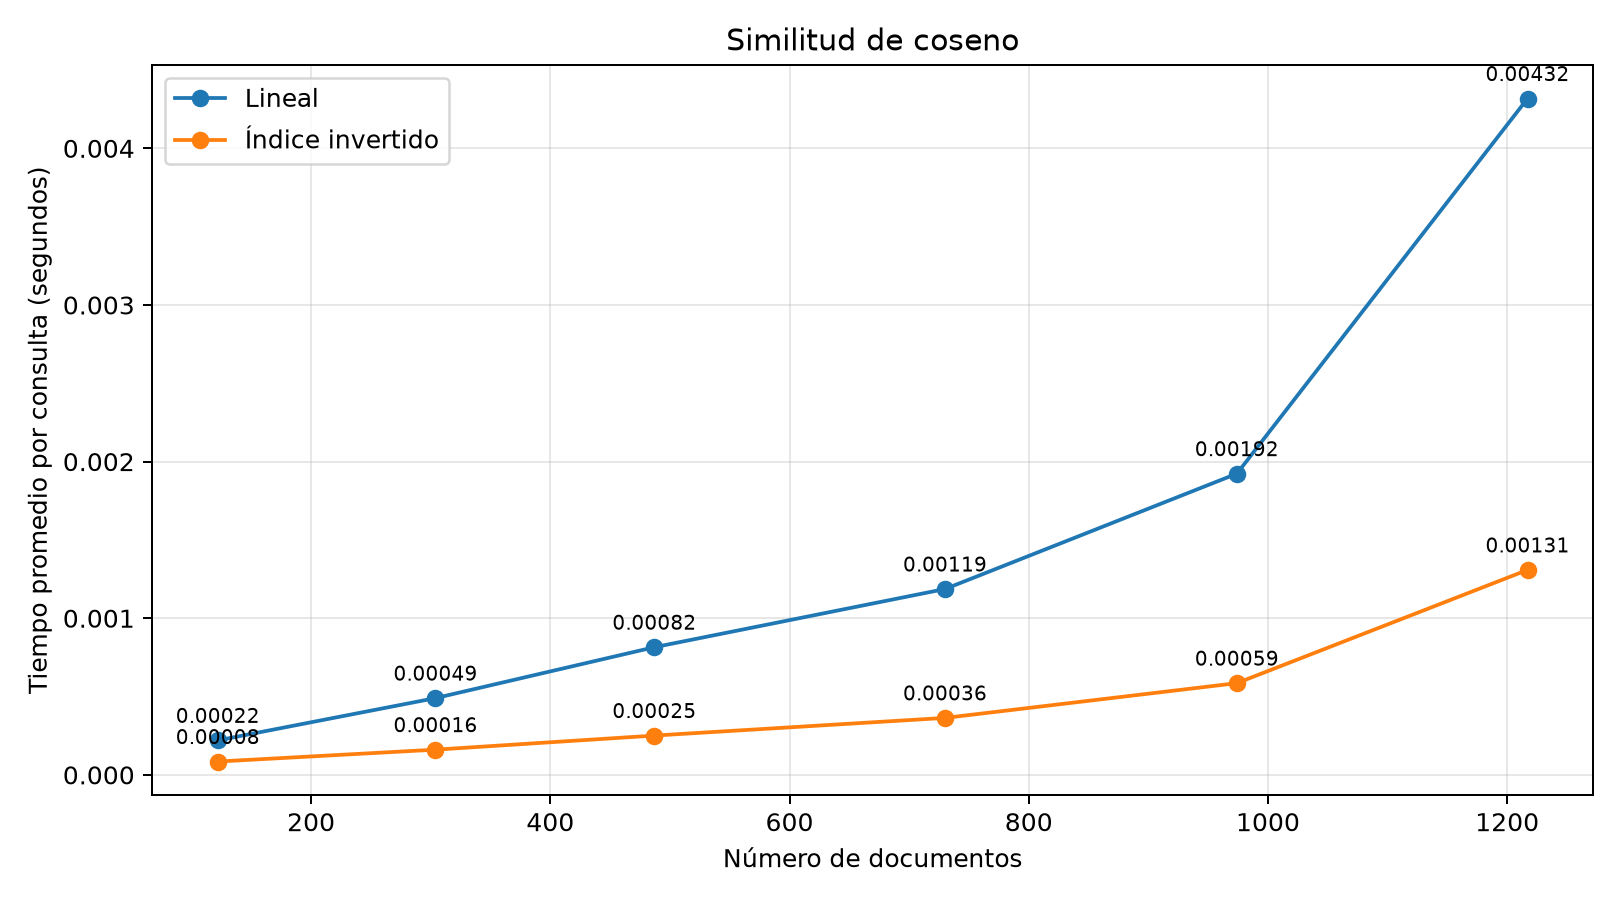
\includegraphics[width=0.95\linewidth]{resultados/coseno.png}
\caption{Tiempo promedio de similitud de coseno; construcción excluida.}
\end{figure}

\section{P6. Análisis de resultados}

La búsqueda booleana lineal recorre todos los documentos y evalúa cada consulta sobre su
diccionario de términos. Para una consulta de longitud fija su costo es $O(N)$; si se
explicita el número $q$ de términos, es $O(Nq)$. La búsqueda booleana con índice lee las
listas de los términos solicitados y combina identificadores ordenados: su costo de
consulta depende de las longitudes de esas listas, aproximadamente
$O(\sum_{t\in Q} |L(t)|)$, más la ordenación de la salida cuando corresponde. No es
independiente de $N$: un término muy común puede producir una lista casi tan grande
como la colección. En 122 documentos medimos 0.000382 s
para el recorrido lineal y 0.000051 s para el índice; en
1217 documentos, 0.004404 s y
0.000441 s, respectivamente. La tendencia favorece al índice,
aunque pequeñas oscilaciones entre tamaños muestran que no debemos interpretar cada
punto como una ley exacta del tiempo de ejecución.

El coseno lineal también visita los $N$ documentos. Con los pesos y normas
precalculados, su trabajo por consulta es $O(Nq)$; el coseno con índice visita solo
las listas de los términos de la consulta y acumula los candidatos, con costo cercano
a $O(\sum_{t\in Q} |L(t)| + C\log C)$ por el ordenamiento de $C$ candidatos.
En 122 documentos sus promedios fueron 0.000220 s y
0.000085 s; en 1217, 0.004318 s y
0.001308 s. En el tamaño mayor, los cocientes lineal/índice
son 9.99 para booleana y 3.30 para coseno. Estos cocientes describen
solo las consultas y la máquina medidas, no una mejora universal.

El primer tamaño ensayado donde el índice ganó fue 122 documentos
para booleana y 122 para coseno. Por tanto, en esta muestra los puntos
observados coinciden; no podemos ubicar un punto de quiebre más preciso por debajo del
primer tamaño. La construcción del índice quedó fuera de las curvas de consulta y se
midió aparte: 0.01200 s para 122 documentos y 0.16528 s para
1217. Para una colección pequeña o una sola consulta, ese costo puede superar el
ahorro de búsqueda. Además, el tiempo de construcción fluctúa por carga del sistema,
asignación de memoria y ejecución de Python; por ello no debe sumarse silenciosamente
a una sola curva. Si se reutiliza el índice para muchas consultas, el costo inicial
se amortiza. El BoW y las estadísticas IDF/norma también se prepararon antes de medir
ambas rutas de coseno, de modo que las curvas comparan únicamente la consulta.

En los seis tamaños, las seis consultas booleanas devolvieron exactamente los mismos
identificadores. Las tres consultas de coseno devolvieron el mismo top 5 en el mismo
orden, con scores iguales dentro de tolerancia absoluta y relativa $10^{-12}$.
No observamos diferencias de ranking ni de resultados. Una variación minúscula de
coma flotante sería posible si cambia el orden de suma: el índice acumula aportes por
lista, mientras el recorrido lineal suma por documento. El desempate fija score
descendente e identificador ascendente. Consultas sin términos compartidos devuelven
una lista vacía y un $k$ mayor que los candidatos devuelve solo los candidatos existentes.

El índice completo contiene 13343 términos distintos y
180216 entradas documento--frecuencia. Si la colección creciera
100 veces con distribución comparable, las entradas podrían acercarse a
18021600, además de diccionarios, cadenas, pesos y texto;
el uso de RAM, las pausas de memoria y el tiempo de reconstrucción serían problemas
prácticos. Una alternativa es guardar las listas invertidas en un índice persistente
en disco, por ejemplo una tabla PostgreSQL de término, documento y frecuencia con
índice B-tree, o un motor de búsqueda especializado. Allí se pueden actualizar
documentos por lotes y consultar sin cargar todas las listas en memoria. La elección
exigiría medir también el costo de E/S y mantenimiento del índice.


\section{Reproducción}
Desde PowerShell, en la carpeta del proyecto, ejecutar en orden:
\begin{verbatim}
.\.venv\Scripts\python.exe crear_bd.py
.\.venv\Scripts\python.exe carga.py
.\.venv\Scripts\python.exe -m unittest -v test_laboratorio.py
.\.venv\Scripts\python.exe ejecutar_lab.py all --repeats 30
.\.venv\Scripts\python.exe generar_informe.py
\end{verbatim}
El primer comando comprueba o crea el esquema; el segundo carga los archivos
si las tablas están vacías; el tercero verifica casos pequeños; el cuarto
actualiza BoW faltantes, comprueba equivalencia y mide; el quinto reconstruye
este informe a partir de los CSV. Para compilar en Overleaf, subir este \codigo{.tex}
y la carpeta \codigo{resultados} con los dos PNG. Los datos crudos y el
script permiten repetir y auditar el experimento.
\end{document}
